\begin{figure}[t]
\eightpoint
\begin{verbatim}
float->float pipeline Main {
  add Source();  // code for Source not shown
  add FIR();
  add Output();  // code for Output not shown
}

float->float filter FIR (float sampRate, int N) {
    float[N] weights;

    init {
        weights = calcImpulseResponse(sampRate, N);
    }

    prework push N-1 pop 0 peek N {
        for (int i=1; i<N; i++) {
            push(doFIR(i));
        }
    }

    work push 1 pop 1 peek N {
        push(doFIR(N));
        pop();
    }

    float doFIR(int k) {
        float val = 0;
        for (int i=0; i<k; i++) {
            val += weights[i] * peek(k-i-1);
        }
        return val;
    }

    handler changeWeights(float[N] newWeights) {
        weights = newWeights;
    }
}
\end{verbatim}

\caption{Example StreamIt program with FIR filter.\protect\label{fig:fir-pipeline}}
\end{figure}

\section{The StreamIt Language}

StreamIt is an architecture-independent language for high-performance
stream programming~\cite{thies-cc02}.  The compiler is publicly
available~\cite{streamitweb} and includes backends for multicore
architectures, clusters of workstations, and Tilera architectures.

The model of computation in StreamIt is grounded in (but not limited
to) synchronous dataflow~\cite{lee87}.  In this model, the programmer
implements independent actors, or {\it filters}, which translate data
items from input channels to output channels.  Filters are composed
into graphs that represent the overall computation.  The key property
of synchronous dataflow is that the number of items consumed and
produced during each execution of a filter is known at compile time,
allowing the compiler to perform static scheduling and optimization.

An example StreamIt program appears in Figure~\ref{fig:fir-pipeline}.
It is based on an FIR filter, which contains three units of execution.
The most important is the {\it work} function, which represents the
steady-state execution step.  Within the work function, a filter may
{\it peek} at a given element on the input tape, {\it pop} an item off
the input tape, or {\it push} an item to the output tape.  The total
number of items peeked, popped, and pushed are declared as part of the
work function.  Note that if the peek rate exceeds the pop rate, it
represents a sliding window computation in which some input elements
are accessed across multiple invocations of the filter.

In addition to the work function, a filter may declare an {\it init}
function to initialize internal data structures, as well as a {\it
  prework} function to perform specialized processing of data items
prior to the steady state.  The prework function is needed in cases
where the initial processing has a different input or output rate than
the steady-state processing.

A {\it schedule} gives a multiplicity for each filter in a stream
graph.  The multiplicity that denotes how many times to fire each
filter where a firing denotes a call to a filter's {\it work} function
(or {\it prework} function on the first iteration of the filter).  The
{\it steady-state schedule} can be calculated such that all filters
fire in the schedule, and the schedule can be repeated
indefinitely~\cite{lee87}.  Steady-state execution of the graph
entails repeating the steady-state schedule for as much input as is
expected.  Execution of the stream graph is conceptually wrapped in an
outer loop that continuously executes the steady-state schedule.  All
the multiplicities of the steady-state can be multiplied by the same
constant $c$, and the result will still be a valid steady-state.  We
call this process {\it increasing} the steady-state of the graph by
$c$.

Furthermore, an {\it initialization} schedule enables the steady-state
schedule in the presence of peeking filters.  An initialization
schedule is required if peeking is present in a graph to enable the
calculation and execution of a steady-state
schedule~\cite{karczmarek-lctes03}.  During application execution, the
{\it init} function is called once for each filter, then the
initialization schedule is executed once, followed by an infinite
repetition of the steady-state schedule.

As depicted in Figure~\ref{fig:structures}, StreamIt provides three
hierarchical primitives for composing filters into stream graphs.  A
{\it pipeline} represents a sequential composition of streams, in
which the output of one stream feeds into the input of the next.  A
{\it splitjoin} represents a parallel set of streams, which divulge
from a common {\it splitter} and converge to a common {\it joiner}.
The types of splitters and joiners are predefined by the StreamIt
language; they encompass duplication and weighted round-robin
behaviors.  Finally, a {\it feedbackloop} represents a cycle in the
stream graph.

\begin{figure}[t!]
\centering
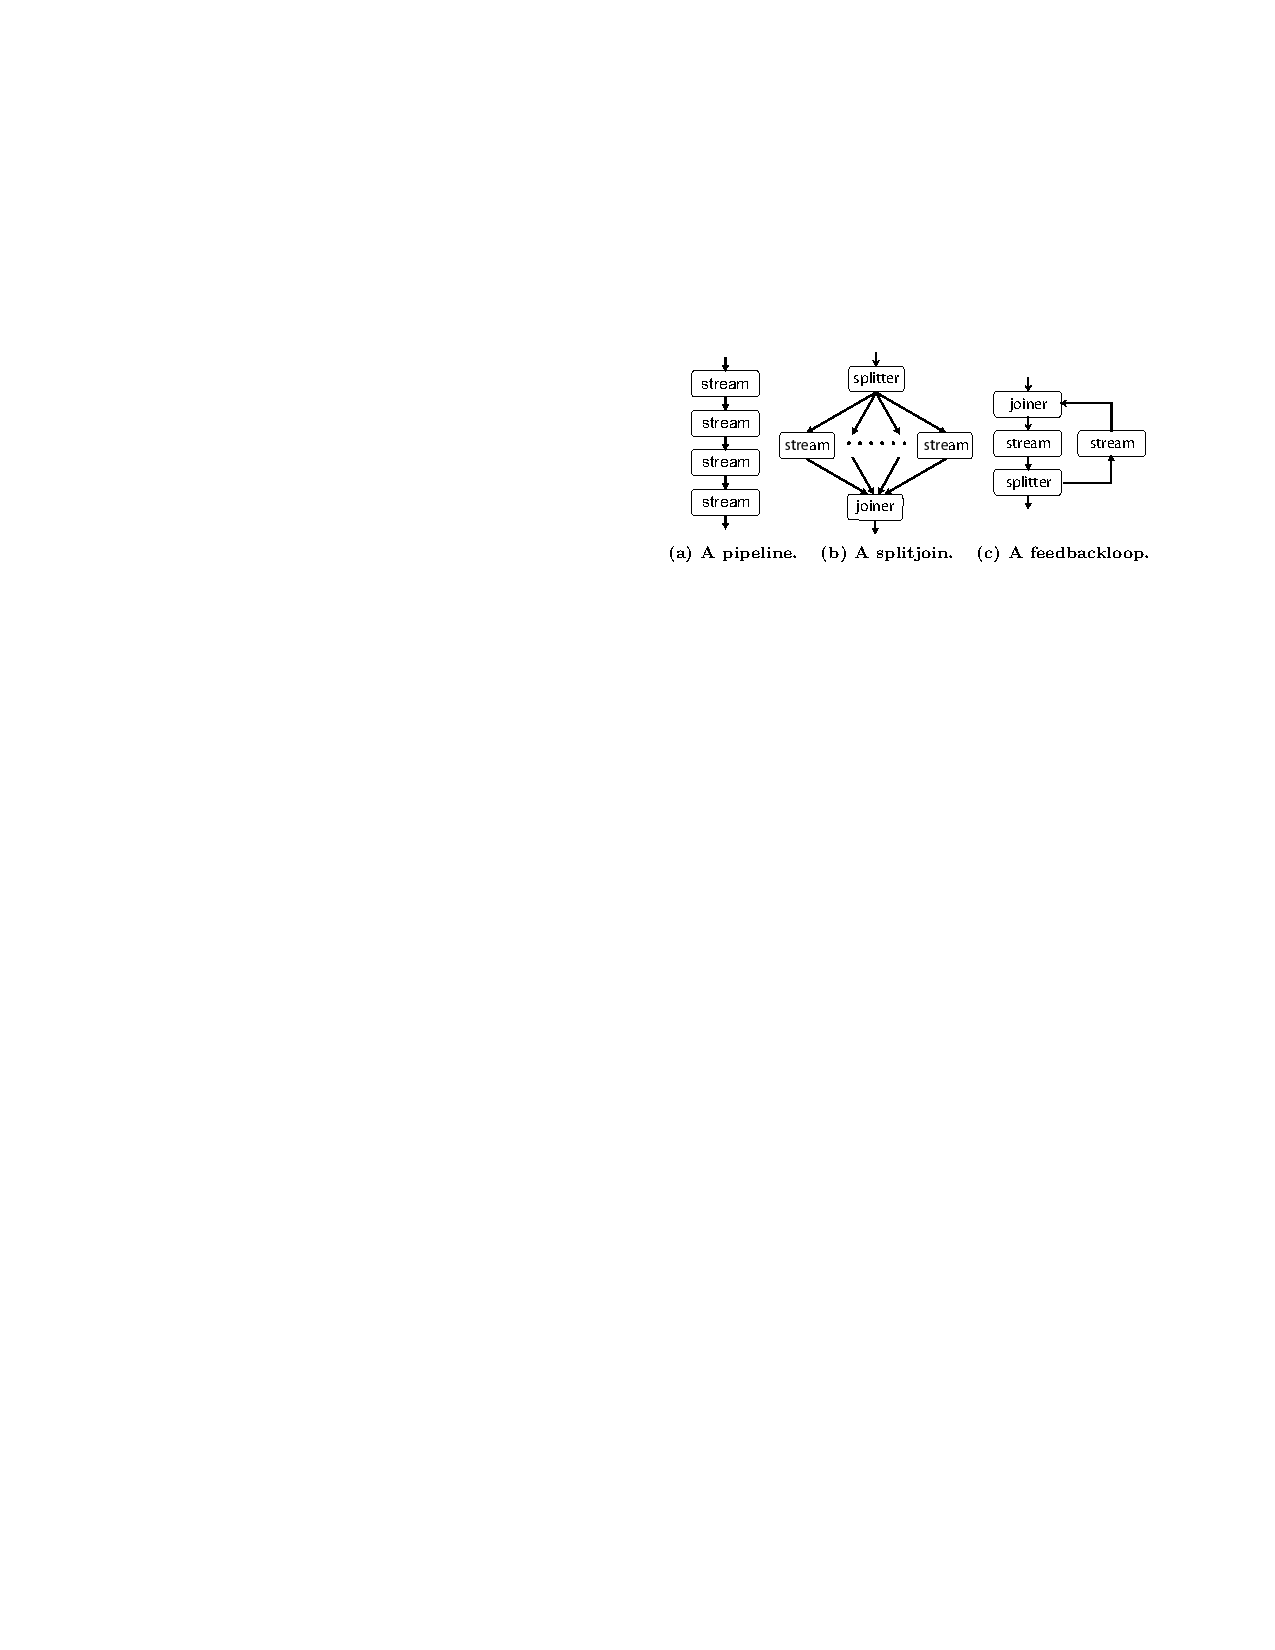
\includegraphics[width=3.3in]{stream-structures.pdf}
%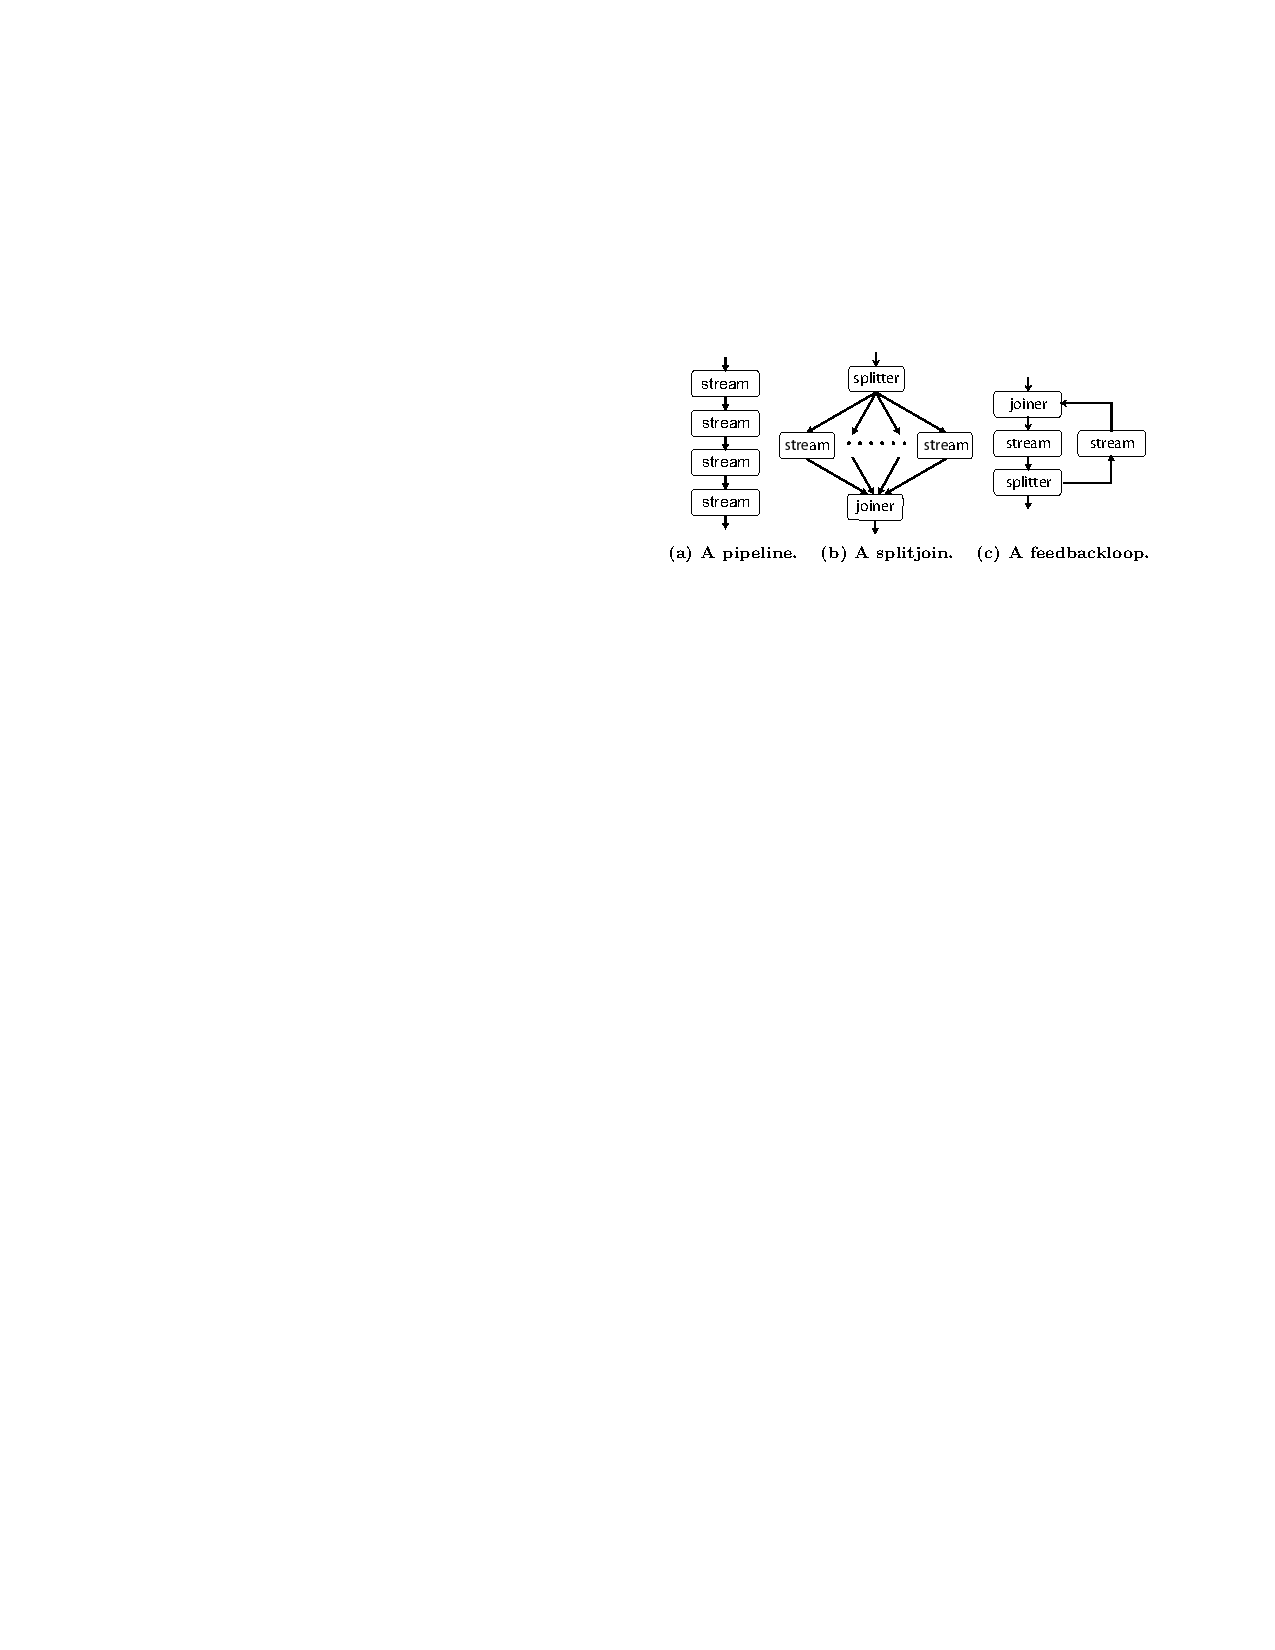
\psfig{file=stream-structures,width=\columnwidth}
\caption{Hierarchical stream structures supported by StreamIt.\protect\label{fig:structures}}
\end{figure}

The StreamIt compiler coarsens the granularity of a stream graph by
applying the {\it fusion} transformation which merges adjacent filters
into a single (large) filter (embedding the schedules of execution in
the merged filter)~\cite{streamit-asplos}.  The {\it fission}
transformation is employed to add data parallelism to a stream graph.
In fission, a single filter without state is duplicated a certain
number of ways and placed in a splitjion construct.  Input items to
the original filter are distributed among the duplicates, termed {\it
  fission products}.  In \S\ref{sec:fission}, we describe how to
extend the fundamental fission transformation to parallelize induction
variable state.
